\documentclass[11pt]{paper}
\usepackage{fullpage}
\usepackage{palatino}
\usepackage{amsfonts,amsmath,amssymb}
% \usepackage{graphicx}

\usepackage{listings}
\usepackage{textcomp}
\usepackage{color}

\definecolor{dkgreen}{rgb}{0,0.6,0}
\definecolor{gray}{rgb}{0.5,0.5,0.5}
\definecolor{mauve}{rgb}{0.58,0,0.82}

\lstset{frame=tb,
  language=R,
  aboveskip=3mm,
  belowskip=3mm,
  showstringspaces=false,
  columns=flexible,
  basicstyle={\small\ttfamily},
  numbers=none,
  numberstyle=\tiny\color{gray},
  keywordstyle=\color{blue},
  commentstyle=\color{dkgreen},
  stringstyle=\color{mauve},
  breaklines=true,
  breakatwhitespace=true,
  tabsize=3
}



\ifx\pdftexversion\undefined
    \usepackage[dvips]{graphicx}
\else
    \usepackage[pdftex]{graphicx}
    \usepackage{epstopdf}
    \epstopdfsetup{suffix=}
\fi

\usepackage{subfig}


% This allows pdflatex to print the curly quotes in the
% significance codes in the output of the GAM.
\UseRawInputEncoding

\begin{document}

%%%%%%%%%%%%%%%%%%%%%%%%%%%%%%%%%%%%%%%%
% Problem Set 7
%%%%%%%%%%%%%%%%%%%%%%%%%%%%%%%%%%%%%%%%

\pagestyle{empty}
{\noindent\bf Spring 2021 \hfill Firstname M.~Lastname}
\vskip 16pt
\centerline{\bf University of Central Florida}
\centerline{\bf College of Business}
\vskip 16pt
\centerline{\bf QMB 6911}
\centerline{\bf Capstone Project in Business Analytics}
\vskip 10pt
\centerline{\bf Solutions:  Problem Set \#9}
\vskip 32pt
\noindent
% 
\section{Data Description}

This analysis follows the script \texttt{Tractor\_Reg\_Model.R} to produce a more accurate model for used tractor prices with the data from \texttt{TRACTOR7.csv} in the \texttt{Data} folder. 
The dataset includes the following variables.
\begin{table}[h!]
\begin{tabular}{l l l}

$saleprice_i$ & = & the price paid for tractor $i$ in dollars \\
% 
$horsepower_i$ & = & the horsepower of tractor $i$ \\
$age_i$ & = & the number of years since tractor $i$ was manufactured  \\
$enghours_i$ & = & the number of hours of use recorded for tractor $i$  \\
$diesel_i$ & = & an indicator of whether tractor $i$ runs on diesel fuel \\ %, $0$ otherwise \\
$fwd_i$ & = & an indicator of whether tractor $i$ has four-wheel drive \\ %, $0$ otherwise \\
$manual_i$ & = & an indicator of whether tractor $i$ has a manual transmission \\ %, $0$ otherwise \\
$johndeere_i$ & = & an indicator of whether tractor $i$ is manufactured by John Deere \\ %, $0$ otherwise \\
$cab_i$ & = & an indicator of whether tractor $i$ has an enclosed cab \\ %, $0$ otherwise \\
% 
$spring_i$ & = & an indicator of whether tractor $i$ was sold in April or May \\ %, $0$ otherwise \\
$summer_i$ & = & an indicator of whether tractor $i$ was sold between June and September \\ %, $0$ otherwise \\
$winter_i$ & = & an indicator of whether tractor $i$ was sold between December and March \\ %, $0$ otherwise \\

\end{tabular}
\end{table}
%

I will revisit the recommended linear model
from Problem Set \#7, 
which included a quadratic specification for horsepower.
This allowed for an increasing relationship 
between price and horsepower, 
for tractors with low horsepower, 
but a decreasing relationship for the tractors with high horsepower. 
I augmented this model in the demonstration for 
Problem Set \#8 
by considering semiparametric specifications
within a Generalized Additive Model. 


Then I will further investigate this nonlinear relationship
by incorporating a nonlinear but parametric specification
for the value of horsepower. 
This parametric analysis will be performed
using the Box-Tidwell framework
to investigate whether the value of these characteristics
are best described with parametric nonlinear forms. 

%%%%%%%%%%%%%%%%%%%%%%%%%%%%%%%%%%%%%%%%
\clearpage
\section{Linear Regression Model}
%%%%%%%%%%%%%%%%%%%%%%%%%%%%%%%%%%%%%%%%

A natural staring point is the recommended linear model
from Problem Set \#7. 

\subsection{Quadratic Specification for Horsepower}

In the demo for Problem Set \#7, 
we considered the advice of
a used tractor dealer who reported that overpowered used tractors are hard to sell, since they consume more fuel. 
This implies that tractor prices often increase with horsepower, up to a point, but beyond that they decrease. 
To incorporate this advice, I created and included a variable for squared horsepower. 
A decreasing relationship for high values of horsepower
is characterized by 
a positive coefficient on the horsepower variable and
a negative coefficient on the squared horsepower variable. 

% 

\begin{table}
\begin{center}
\begin{tabular}{l c c c}
\hline
 & Model 1 & Model 2 & Model 3 \\
\hline
(Intercept)         & $8.60684^{***}$  & $8.72555^{***}$  & $8.72792^{***}$  \\
                    & $(0.11233)$      & $(0.11156)$      & $(0.10602)$      \\
horsepower          & $0.01504^{***}$  & $0.01115^{***}$  & $0.01112^{***}$  \\
                    & $(0.00097)$      & $(0.00107)$      & $(0.00107)$      \\
squared\_horsepower & $-0.00002^{***}$ & $-0.00001^{***}$ & $-0.00001^{***}$ \\
                    & $(0.00000)$      & $(0.00000)$      & $(0.00000)$      \\
age                 & $-0.03429^{***}$ & $-0.03206^{***}$ & $-0.03233^{***}$ \\
                    & $(0.00374)$      & $(0.00359)$      & $(0.00358)$      \\
enghours            & $-0.00004^{***}$ & $-0.00004^{***}$ & $-0.00004^{***}$ \\
                    & $(0.00001)$      & $(0.00001)$      & $(0.00001)$      \\
diesel              & $0.20070^{*}$    & $0.21453^{*}$    & $0.20350^{*}$    \\
                    & $(0.09975)$      & $(0.09854)$      & $(0.09805)$      \\
fwd                 & $0.31288^{***}$  & $0.27526^{***}$  & $0.26539^{***}$  \\
                    & $(0.06259)$      & $(0.05876)$      & $(0.05820)$      \\
johndeere           & $0.23842^{**}$   & $0.30972^{***}$  & $0.31872^{***}$  \\
                    & $(0.07705)$      & $(0.07236)$      & $(0.07186)$      \\
manual              &                  & $-0.15308^{*}$   & $-0.15015^{*}$   \\
                    &                  & $(0.06209)$      & $(0.06189)$      \\
cab                 &                  & $0.47786^{***}$  & $0.48345^{***}$  \\
                    &                  & $(0.07031)$      & $(0.07003)$      \\
spring              &                  & $-0.04892$       &                  \\
                    &                  & $(0.06506)$      &                  \\
summer              &                  & $-0.05729$       &                  \\
                    &                  & $(0.06379)$      &                  \\
winter              &                  & $0.04596$        &                  \\
                    &                  & $(0.07141)$      &                  \\
\hline
R$^2$               & $0.76838$        & $0.80761$        & $0.80591$        \\
Adj. R$^2$          & $0.76233$        & $0.79884$        & $0.79935$        \\
Num. obs.           & $276$            & $276$            & $276$            \\
\hline
\multicolumn{4}{l}{\scriptsize{$^{***}p<0.001$; $^{**}p<0.01$; $^{*}p<0.05$}}
\end{tabular}
\caption{Quadratic Models for Tractor Prices}
\label{tab:reg_sq_horse}
\end{center}
\end{table}

% 
The results of this regression specification are shown in 
Table \ref{tab:reg_sq_horse}. 
%
The squared horsepower variable has a coefficient of $-2.081e-05$, which is nearly ten times as large as the standard error of $2.199e-06$, which is very strong evidence against the null hypothesis of a positive or zero coefficient. 
I conclude that the log of the sale price does decline for large values of horsepower. 


With the squared horsepower variable, the $\bar{R}^2$ is $0.764$, indicating that it is a much stronger model than the others we considered. 
The $F$-statistic is large, indicating that it is a better candidate than the simple average log sale price. 
The new squared horsepower variable is statistically significant and the theory behind it is sound, since above a certain point, added horsepower may not improve performance but will cost more to operate. 
This new model is much improved over the previous models with a linear specification for horsepower.
Next, I will attempt to improve on this specification, 
as we did for Problem Set \#8. 





%%%%%%%%%%%%%%%%%%%%%%%%%%%%%%%%%%%%%%%%
\clearpage
\section{Nonlinear Specifications}
%%%%%%%%%%%%%%%%%%%%%%%%%%%%%%%%%%%%%%%%


% \clearpage
\subsection{Nonparametric Specification for Horsepower}


The specification in 
Table \ref{tab:reg_sq_horse}
assumes a quadratic functional form for
the relationship between price and horsepower. 
To consider the horsepower variable alone, 
while accounting for the effects of other variables, 
one can fit a nonparametric model to the residuals 
from a model of tractor prices, 
after regressing tractor prices on the other variables. 
This leaves only the variation in tractor prices that is not explained by the other variables. 
Going one step further, perform the same transformation to the horsepower variable:
take the residuals from a model of horsepower, 
after regressing horsepower on the other variables. 
This allows a model that would fit exactly the same as if it were estimated within a full model with all variables included. 

I first conducted FWL regressions 
to reduce the problem to two dimensions. 
The results are not shown here, 
since the comparison only verifies 
the conclusion of the FWL theorem. 


% \clearpage
To illustrate the fit of the model, 
\ref{fig:dev_vs_horse_dev} 
shows a scatter plot 
of the residual log prices on 
residuals from the regression for horsepower:
the ``excess horsepower'' compared to what would be 
expected given the other characteristics of a tractor. 
The observations are shown in blue
and the fitted values are shown in red.
The quadratic function is clear from this perspective, 
except that we observe variation in the fitted values results from the 
two-dimensional nature of the horsepower variable
when we consider the quadratic form.

I next considered a nonparametric specification for 
the relationship between prices and horsepower.
Figure \ref{fig:dev_np_vs_horse_dev} 
overlays the nonparametric estimate (shown in green) 
compared to the linear model.
The pattern has more variation in slope but 
closely follows the prediction from the quadratic model. 
So far, it appears that the quadratic form
is close enough.

\begin{figure}[h!]
  \centering
  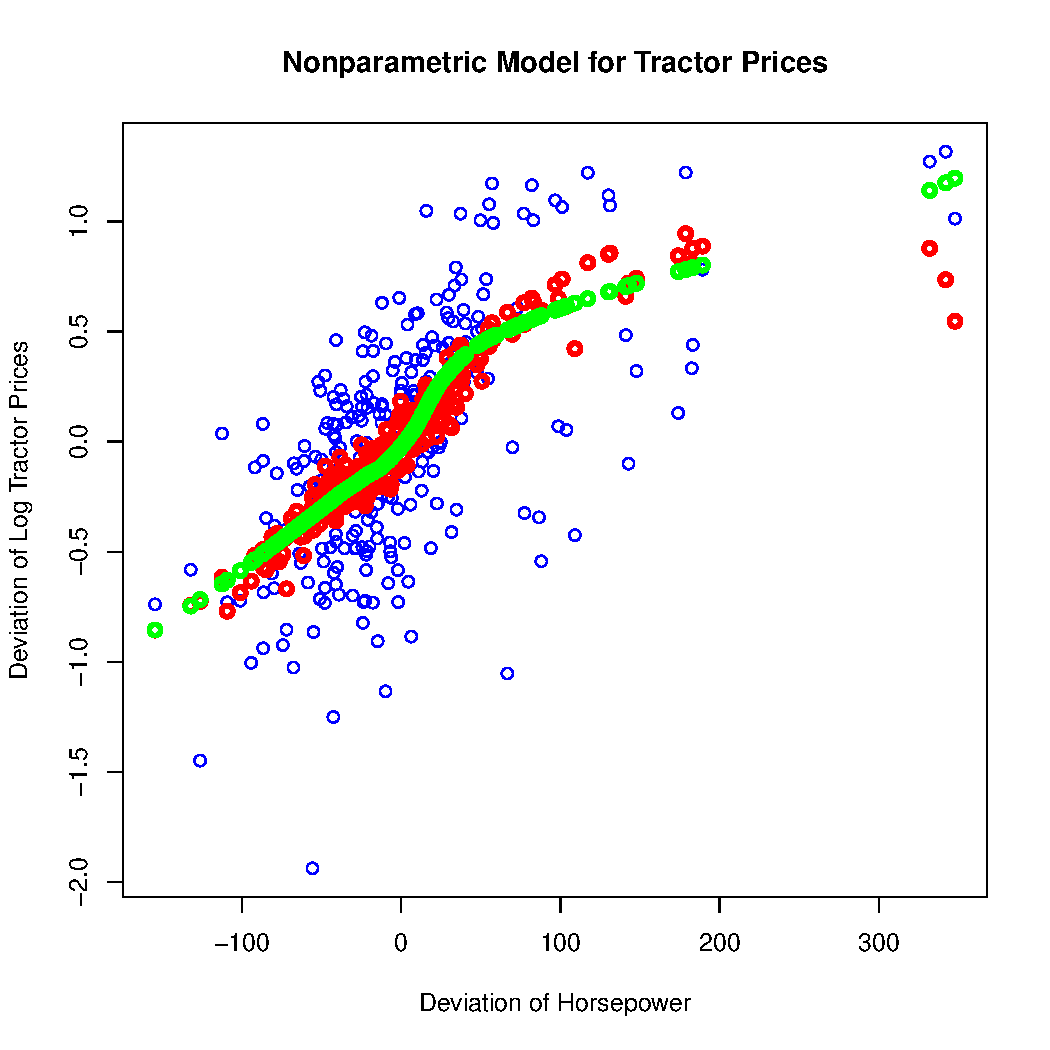
\includegraphics[scale = 0.5, keepaspectratio=true]{../Figures/dev_np_vs_horse_dev}
  \caption{Nonparametric Model for Tractor Prices: Excess Horsepower} \label{fig:dev_np_vs_horse_dev}
\end{figure}

 


\clearpage
\subsection{Nonparametric Specification for Age}

As above, first conduct FWL regressions 
to reduce the problem to two dimensions. 
% 
To illustrate the fit of the model, 
Figure \ref{fig:dev_np_vs_age_dev} 
shows a scatter plot 
of the residual log prices on 
the residuals from the regression for age:
the ``excess age'' of a tractor compared to what would be 
expected given the other characteristics of the tractor. 
% 
The observations are shown in blue
and the fitted values are shown in red.

Next we considered a nonparametric specification for 
the relationship between prices and age.
% 
Figure \ref{fig:dev_np_vs_age_dev} 
overlays the nonparametric estimate (shown in green) 
with the linear model.
The pattern has more variation in slope but 
closely follows the prediction from the linear model. 
Although the nonparametric estimate varies around the linear estimate,
it appears that the linear form
is a close enough approximation without the added complexity.
Next, I will revisit the remaining continuous variable.


\begin{figure}[h!]
  \centering
  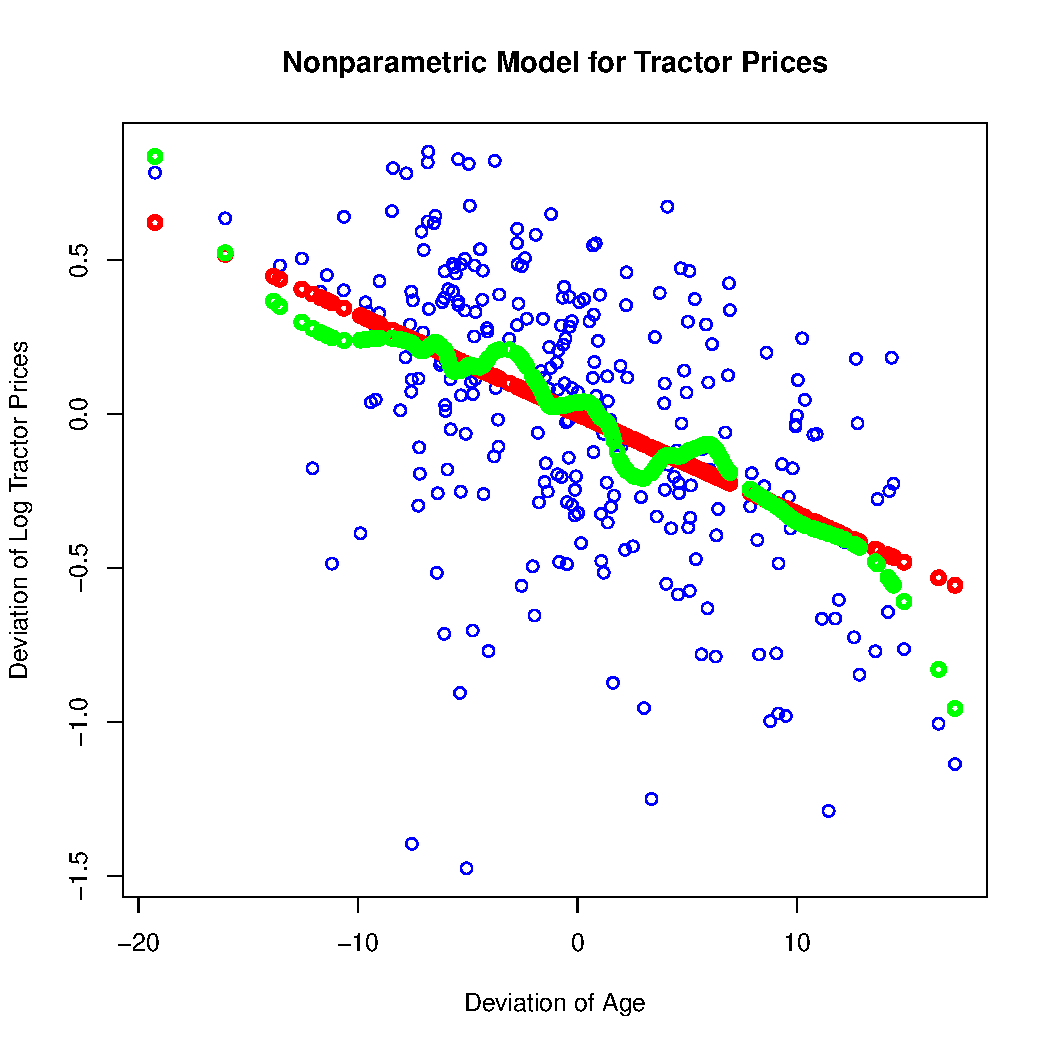
\includegraphics[scale = 0.5, keepaspectratio=true]{../Figures/dev_np_vs_age_dev}
  \caption{Nonparametric Model for Tractor Prices: Excess Age} \label{fig:dev_np_vs_age_dev}
\end{figure}





\clearpage
\subsection{Nonparametric Specification for Engine Hours}

As above, first conduct FWL regressions 
to reduce the problem to two dimensions. 
%
To illustrate the fit of the model, 
Figure \ref{fig:dev_np_vs_eng_dev}
shows a scatter plot 
of the residual log prices on 
residuals from the regression for engine hours:
the ``excess engine hours'' of a tractor compared to what would be 
expected given the other characteristics of the tractor. 
The observations are shown in blue
and the fitted values are shown in red.
As with age, the linear fit follows a straight line,
since we have a single variable with no
quadratic transformation.
% 
I moved directly to the nonparametric specification for 
the relationship between prices and engine hours.
Figure \ref{fig:dev_np_vs_eng_dev} 
overlays the nonparametric estimate, shown in green. 
The pattern has more variation in slope but 
closely follows the prediction from the linear model. 
Although the nonparametric estimate varies around the linear estimate,
it appears that the linear form
is also a close enough approximation, 
just as was found for the age variable.


\begin{figure}[h!]
  \centering
  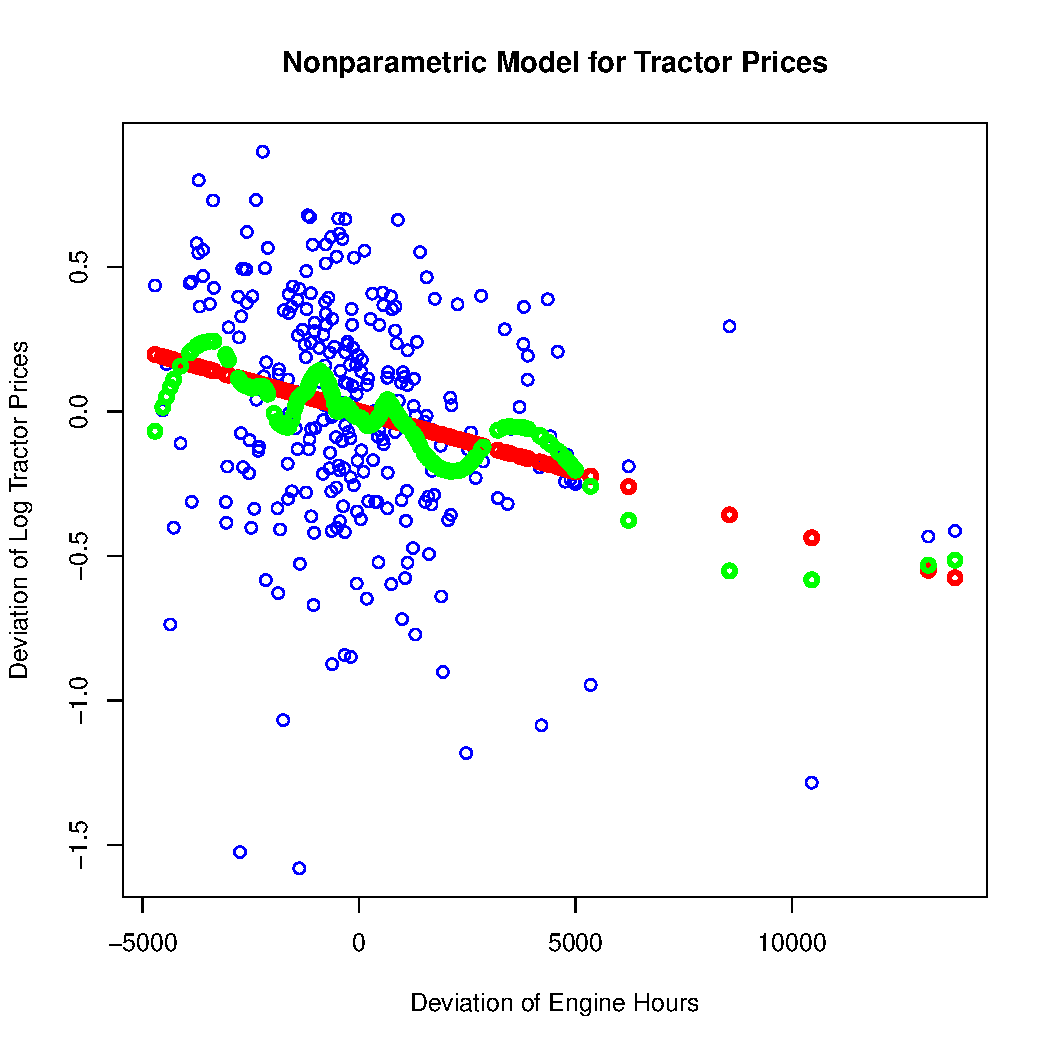
\includegraphics[scale = 0.5, keepaspectratio=true]{../Figures/dev_np_vs_eng_dev}
  \caption{Nonparametric Model for Tractor Prices: Excess Engine Hours} \label{fig:dev_np_vs_eng_dev}
\end{figure}

 

\pagebreak
\section{Semiparametric Estimates}

As I was building the above nonparametric models, 
I stored the predictions and will now use them as variables in 
linear models. 
Table \ref{tab:reg_semipar} 
shows the estimates from a set of models. 
Model 1 is the benchmark linear model in 
Table \ref{tab:reg_sq_horse}. 
Model 2 is a semi-parametric model
with a nonparametric fit on horsepower
substituted in for the horsepower variables.
Models 3 and 4 are semi-parametric models
with nonparametric fits on age and engine hours, respectively.
Model 5 is a maximally semiparametric model, 
with nonparametric fits for all continuous variables. 
For each of the single-variable semiparametric models, 
the coefficients are near one
and the fits are similar to the linear model. 
Even with maximal flexibility, the fit of Model 5
is not much better than the benchmark linear model. 
Across all models, the adjusted $\bar{R}^2$ values are all hovering around 0.80. 
All things considered, these are excellent models
and the linear model is sufficient.


\begin{table}
\begin{center}
\begin{tabular}{l c c c c c}
\hline
 & Model 1 & Model 2 & Model 3 & Model 4 & Model 5 \\
\hline
(Intercept)                 & $2.00999^{***}$ & $2.34926^{***}$ & $2.98091^{***}$  & $3.23438^{***}$ & $4.49531^{***}$  \\
                            & $(0.26125)$     & $(0.22596)$     & $(0.22704)$      & $(0.15261)$     & $(0.05897)$      \\
Width                       & $0.33575^{*}$   &                 & $0.92791^{***}$  & $0.03044$       &                  \\
                            & $(0.15622)$     &                 & $(0.12784)$      & $(0.14082)$     &                  \\
Diameter                    & $0.39567^{***}$ & $0.43144^{***}$ &                  & $0.33658^{***}$ &                  \\
                            & $(0.05076)$     & $(0.04150)$     &                  & $(0.04671)$     &                  \\
Density                     & $1.21296^{***}$ & $1.07566^{***}$ & $0.81613^{***}$  &                 &                  \\
                            & $(0.21948)$     & $(0.20093)$     & $(0.20645)$      &                 &                  \\
SealedYes                   & $0.62731^{***}$ & $0.61960^{***}$ & $0.70050^{***}$  & $0.56858^{***}$ & $0.69858^{***}$  \\
                            & $(0.08622)$     & $(0.08246)$     & $(0.08226)$      & $(0.08047)$     & $(0.07509)$      \\
MachinedYes                 & $0.64934^{***}$ & $0.58954^{***}$ & $0.71659^{***}$  & $0.65070^{***}$ & $0.61103^{***}$  \\
                            & $(0.08320)$     & $(0.07933)$     & $(0.07938)$      & $(0.07819)$     & $(0.07386)$      \\
made\_in\_USATRUE           & $0.74633^{***}$ & $0.77354^{***}$ & $0.79615^{***}$  & $0.70473^{***}$ & $0.79326^{***}$  \\
                            & $(0.09247)$     & $(0.08855)$     & $(0.08879)$      & $(0.08692)$     & $(0.08296)$      \\
SealedYes:made\_in\_USATRUE & $-0.29519^{**}$ & $-0.29826^{**}$ & $-0.33376^{***}$ & $-0.27253^{**}$ & $-0.31356^{***}$ \\
                            & $(0.10092)$     & $(0.09642)$     & $(0.09694)$      & $(0.09500)$     & $(0.09038)$      \\
width\_np                   &                 & $1.11995^{***}$ &                  &                 & $1.35512^{***}$  \\
                            &                 & $(0.21565)$     &                  &                 & $(0.20456)$      \\
diameter\_np                &                 &                 & $1.00650^{***}$  &                 & $1.00083^{***}$  \\
                            &                 &                 & $(0.10926)$      &                 & $(0.10411)$      \\
density\_np                 &                 &                 &                  & $1.03923^{***}$ & $0.76790^{***}$  \\
                            &                 &                 &                  & $(0.12864)$     & $(0.12582)$      \\
\hline
R$^2$                       & $0.74893$       & $0.76995$       & $0.76755$        & $0.77748$       & $0.79771$        \\
Adj. R$^2$                  & $0.74160$       & $0.76324$       & $0.76077$        & $0.77099$       & $0.79181$        \\
Num. obs.                   & $248$           & $248$           & $248$            & $248$           & $248$            \\
\hline
\multicolumn{6}{l}{\scriptsize{$^{***}p<0.001$; $^{**}p<0.01$; $^{*}p<0.05$}}
\end{tabular}
\caption{Semiparametric Models for Fly Reel Prices}
\label{tab:reg_semipar}
\end{center}
\end{table}






\pagebreak
\section{Generalized Additive Model}

\subsection{Linear Model}

As an example of the output from the GAM specification, 
I first estimated the model with no nonlinear terms, 
which is essentially a linear regression. 

\begin{verbatim}
Family: gaussian 
Link function: identity 

Formula:
log_Price ~ Width + Diameter + Density + Sealed + Machined + 
    made_in_USA + made_in_USA * Sealed

Parametric coefficients:
                          Estimate Std. Error t value Pr(>|t|)    
(Intercept)                2.00999    0.26125   7.694 3.69e-13 ***
Width                      0.33575    0.15622   2.149  0.03262 *  
Diameter                   0.39567    0.05076   7.795 1.95e-13 ***
Density                    1.21296    0.21948   5.527 8.49e-08 ***
SealedYes                  0.62731    0.08622   7.275 4.88e-12 ***
MachinedYes                0.64934    0.08320   7.805 1.84e-13 ***
made_in_USATRUE            0.74633    0.09247   8.071 3.35e-14 ***
SealedYes:made_in_USATRUE -0.29519    0.10092  -2.925  0.00378 ** 
---
Signif. codes:  0 �***� 0.001 �**� 0.01 �*� 0.05 �.� 0.1 � � 1


R-sq.(adj) =  0.742   Deviance explained = 74.9%
GCV = 0.10913  Scale est. = 0.10561   n = 248
\end{verbatim}

\pagebreak
\subsection{Semiparametric Model}


Further investigating the results of the full semiparametric specification
in Model 5 of Table \ref{tab:reg_semipar},
I estimated the model with all three continuous variables specified as nonparametric functions. 
The result was that 
almost all the variables---both linear and nonlinear---were 
statistically significant. 
The only exception was a loss in significance of the diesel indicator. 


\begin{verbatim}
Family: gaussian 
Link function: identity 

Formula:
log_saleprice ~ s(horsepower) + s(age) + s(enghours) + diesel + 
    fwd + manual + johndeere + cab

Parametric coefficients:
            Estimate Std. Error t value Pr(>|t|)    
(Intercept)  9.04516    0.09366  96.575  < 2e-16 ***
diesel       0.13440    0.09499   1.415  0.15830    
fwd          0.29899    0.05754   5.196 4.11e-07 ***
manual      -0.16938    0.05965  -2.839  0.00487 ** 
johndeere    0.33067    0.06890   4.799 2.68e-06 ***
cab          0.40439    0.07151   5.655 4.08e-08 ***
---
Signif. codes:  0 �***� 0.001 �**� 0.01 �*� 0.05 �.� 0.1 � � 1

Approximate significance of smooth terms:
                edf Ref.df     F  p-value    
s(horsepower) 4.387  5.321 44.89  < 2e-16 ***
s(age)        3.264  4.057 21.59  < 2e-16 ***
s(enghours)   1.000  1.000 23.39 2.64e-06 ***
---
Signif. codes:  0 �***� 0.001 �**� 0.01 �*� 0.05 �.� 0.1 � � 1

R-sq.(adj) =  0.819   Deviance explained = 82.8%
GCV = 0.15063  Scale est. = 0.14263   n = 276
\end{verbatim}

On the other hand, 
the adjusted R-squared has not increased very much, 
from 0.799 to 0.819 under this specification, 
which may not justify the added complexity of the model.
Perhaps more importantly, the coefficients on the 
linear terms are very similar across models, 
indicating that the models support similar conclusions relating to any business decision involving
the John Deere premium. 
With this second model, we have even more support for those conclusions
and are certain that the conclusions are not 
coincidental results of the
functional form decisions for previous models.


Perhaps as a middle ground, we can estimate a model with a 
nonparametric specification for the horsepower variable alone, 
since it seems to have a nonlinear relationship with value in either case. 
This retains most of the predictive value of the maximally 
semiparametric model and accommodates the 
nonlinear relationship with value of horsepower. 

\begin{verbatim}
Family: gaussian 
Link function: identity 

Formula:
log_saleprice ~ s(horsepower) + age + enghours + diesel + fwd + 
    manual + johndeere + cab

Parametric coefficients:
              Estimate Std. Error t value Pr(>|t|)    
(Intercept)  9.697e+00  1.120e-01  86.607  < 2e-16 ***
age         -3.114e-02  3.539e-03  -8.799  < 2e-16 ***
enghours    -4.354e-05  9.342e-06  -4.660 5.02e-06 ***
diesel       1.372e-01  9.590e-02   1.431  0.15361    
fwd          3.134e-01  5.773e-02   5.428 1.29e-07 ***
manual      -1.650e-01  6.041e-02  -2.732  0.00673 ** 
johndeere    3.189e-01  6.933e-02   4.599 6.59e-06 ***
cab          3.770e-01  7.202e-02   5.235 3.38e-07 ***
---
Signif. codes:  0 ‘***’ 0.001 ‘**’ 0.01 ‘*’ 0.05 ‘.’ 0.1 ‘ ’ 1

Approximate significance of smooth terms:
                edf Ref.df     F p-value    
s(horsepower) 4.758  5.751 44.49  <2e-16 ***
---
Signif. codes:  0 ‘***’ 0.001 ‘**’ 0.01 ‘*’ 0.05 ‘.’ 0.1 ‘ ’ 1

R-sq.(adj) =  0.815   Deviance explained = 82.3%
GCV = 0.15323  Scale est. = 0.14615   n = 276
\end{verbatim}


\pagebreak
\section{The Box--Tidwell Transformation}

The Box--Tidwell function tests for non-linear relationships
to the mean of the dependent variable.
The nonlinearity is in the form of an
exponential transformation in the form of the Box-Cox
transformation, except that the transformation is taken
on the explanatory variables.


\subsection{Transformation of Horsepower}


Performing the transformation on the horsepower variable
produces a modified form of the linear model.
This specification allows a single exponential
transformation on horsepower, rather than a quadratic form.

\begin{verbatim} MLE of lambda Score Statistic (z)  Pr(>|z|)    
       0.11437             -7.3864 1.509e-13 ***
---
Signif. codes:  0 ‘***’ 0.001 ‘**’ 0.01 ‘*’ 0.05 ‘.’ 0.1 ‘ ’ 1

iterations =  5 
\end{verbatim}

The \textsf{R} output is the statistics for a test of nonlinearity:
that the exponent $\lambda$ in the Box--Tidwell transformation is zero.
%
The "\texttt{MLE of lambda}" statistic is the optimal exponent on horsepower.
Similar to the Box-Cox transformation,
with Box-Tidwell, the exponents are on the explanatory variables
and are all called lambda, in contrast
to the parameter $\tau$ in our class notes.
The exponent is significantly different from 0,
although it is a small positive value,
which suggests an increasing relationship
for the value of horsepower
with a slope that is sharply declining.
Next I consider the possibility of a changing relationship 
for the next continuous variable. 


\subsection{Transformation of Age}


\begin{verbatim} MLE of lambda Score Statistic (z) Pr(>|z|)
        0.9815              0.0421   0.9664

iterations =  3 
\end{verbatim}

This coefficient is effectively 1, which is more evidence of
a purely linear relationship between \texttt{log\_saleprice}
and age: the percentage depreciation rate is constant.
Next, I will consider the possibility of nonlinearity 
in depreciation from hours of use. 

\subsection{Transformation of Engine Hours}


\begin{verbatim} MLE of lambda Score Statistic (z) Pr(>|z|)
        1.3578             -0.9646   0.3348

iterations =  3 
\end{verbatim}

Although $\hat{\lambda}$ is not statistically significant,
this suggests a moderately increasing relationship
between the log of tractor prices and engine hours,
which means that tractors with high hours of use
depreciate more quickly with each additional hour of use.

Since a nonlinear relationship was detected with horsepower,
I will next estimate a model
with nonlinearity in all three continuous variables.


\subsection{Transformation of All Three Continuous Variables}


\begin{verbatim}           MLE of lambda Score Statistic (z)  Pr(>|z|)    
horsepower        0.1153             -7.1510 8.615e-13 ***
age               1.1183             -0.0489    0.9610    
enghours          1.1043             -0.5379    0.5907    
---
Signif. codes:  0 ‘***’ 0.001 ‘**’ 0.01 ‘*’ 0.05 ‘.’ 0.1 ‘ ’ 1

iterations =  6 
\end{verbatim}


The performance is similar to the other models with
forms of nonlinearity for the value of horsepower.
Now consider the full set of such models in a table for a final comparison.


\pagebreak
\section{Final Comparison of Candidate Models}

I created one more variable \texttt{horsepower\_bt}
by raising horsepower to the optimal exponent 
$\hat{\lambda} = 0.1143693$. 
Then, I included this variable in the place of 
the horsepower variables a the linear regression model.
% 
Table \ref{tab:reg_sq_horse_sp_bt} collects the results
of the set of models from the three forms of nonlinearity.
Model 1 is the linear regression model with 
a quadratic form for horsepower. 
Model 2 is the semiparametric model with
a nonparametric form for horsepower. 
Model 3 has the same specification as the other two, 
except that the horsepower variable is transformed using the optimal
exponent for the Box-Tidwell transformation. 
% 
The last model has the highest R-squared
among the ones we have estimated.
Again, the differences are marginal, so the practical recommendation
is the model with the quadratic relationship for horsepower, 
which has a simpler interpretation.
In either case, we conclude that John Deere tractors are worth
approximately thirty percent more valuable
than an equivalent tractor of another brand. 


\begin{table}
\begin{center}
\begin{tabular}{l c c c}
\hline
 & Model 1 & Model 2 & Model 3 \\
\hline
(Intercept)         & $8.72792^{***}$  & $8.97543^{***}$  & $3.09024^{***}$  \\
                    & $(0.10602)$      & $(0.10479)$      & $(0.39174)$      \\
horsepower          & $0.01112^{***}$  &                  &                  \\
                    & $(0.00107)$      &                  &                  \\
squared\_horsepower & $-0.00001^{***}$ &                  &                  \\
                    & $(0.00000)$      &                  &                  \\
age                 & $-0.03233^{***}$ & $-0.03813^{***}$ & $-0.02927^{***}$ \\
                    & $(0.00358)$      & $(0.00360)$      & $(0.00345)$      \\
enghours            & $-0.00004^{***}$ & $0.00000$        & $-0.00005^{***}$ \\
                    & $(0.00001)$      & $(0.00001)$      & $(0.00001)$      \\
diesel              & $0.20350^{*}$    & $0.31981^{**}$   & $0.12070$        \\
                    & $(0.09805)$      & $(0.09872)$      & $(0.09500)$      \\
fwd                 & $0.26539^{***}$  & $0.39101^{***}$  & $0.32602^{***}$  \\
                    & $(0.05820)$      & $(0.05901)$      & $(0.05617)$      \\
manual              & $-0.15015^{*}$   & $-0.06208$       & $-0.20053^{**}$  \\
                    & $(0.06189)$      & $(0.06285)$      & $(0.06031)$      \\
johndeere           & $0.31872^{***}$  & $0.40778^{***}$  & $0.33386^{***}$  \\
                    & $(0.07186)$      & $(0.07313)$      & $(0.06967)$      \\
cab                 & $0.48345^{***}$  & $1.05513^{***}$  & $0.42139^{***}$  \\
                    & $(0.07003)$      & $(0.05806)$      & $(0.06768)$      \\
horsepower\_np      &                  & $0.96671^{***}$  &                  \\
                    &                  & $(0.06886)$      &                  \\
horsepower\_bt      &                  &                  & $3.99759^{***}$  \\
                    &                  &                  & $(0.25577)$      \\
\hline
R$^2$               & $0.80591$        & $0.79743$        & $0.81613$        \\
Adj. R$^2$          & $0.79935$        & $0.79136$        & $0.81062$        \\
Num. obs.           & $276$            & $276$            & $276$            \\
\hline
\multicolumn{4}{l}{\scriptsize{$^{***}p<0.001$; $^{**}p<0.01$; $^{*}p<0.05$}}
\end{tabular}
\caption{Alternate Models for Tractor Prices}
\label{tab:reg_sq_horse_sp_bt}
\end{center}
\end{table}




%%%%%%%%%%%%%%%%%%%%%%%%%%%%%%%%%%%%%%%%
\end{document}
%%%%%%%%%%%%%%%%%%%%%%%%%%%%%%%%%%%%%%%%
